\documentclass{standalone}
%
\usepackage{tikz}
\usetikzlibrary{backgrounds}
\usepackage{tkz-euclide}
\usetkzobj{all}
%
\usepackage{xcolor}
%
\definecolor{space}{HTML}{1F2C4E}
\definecolor{moon}{HTML}{AFAFAF}
\definecolor{craterm}{HTML}{616060}
\definecolor{linem}{HTML}{DBDBDB}
%
\title{SuperMoon}
\begin{document}
	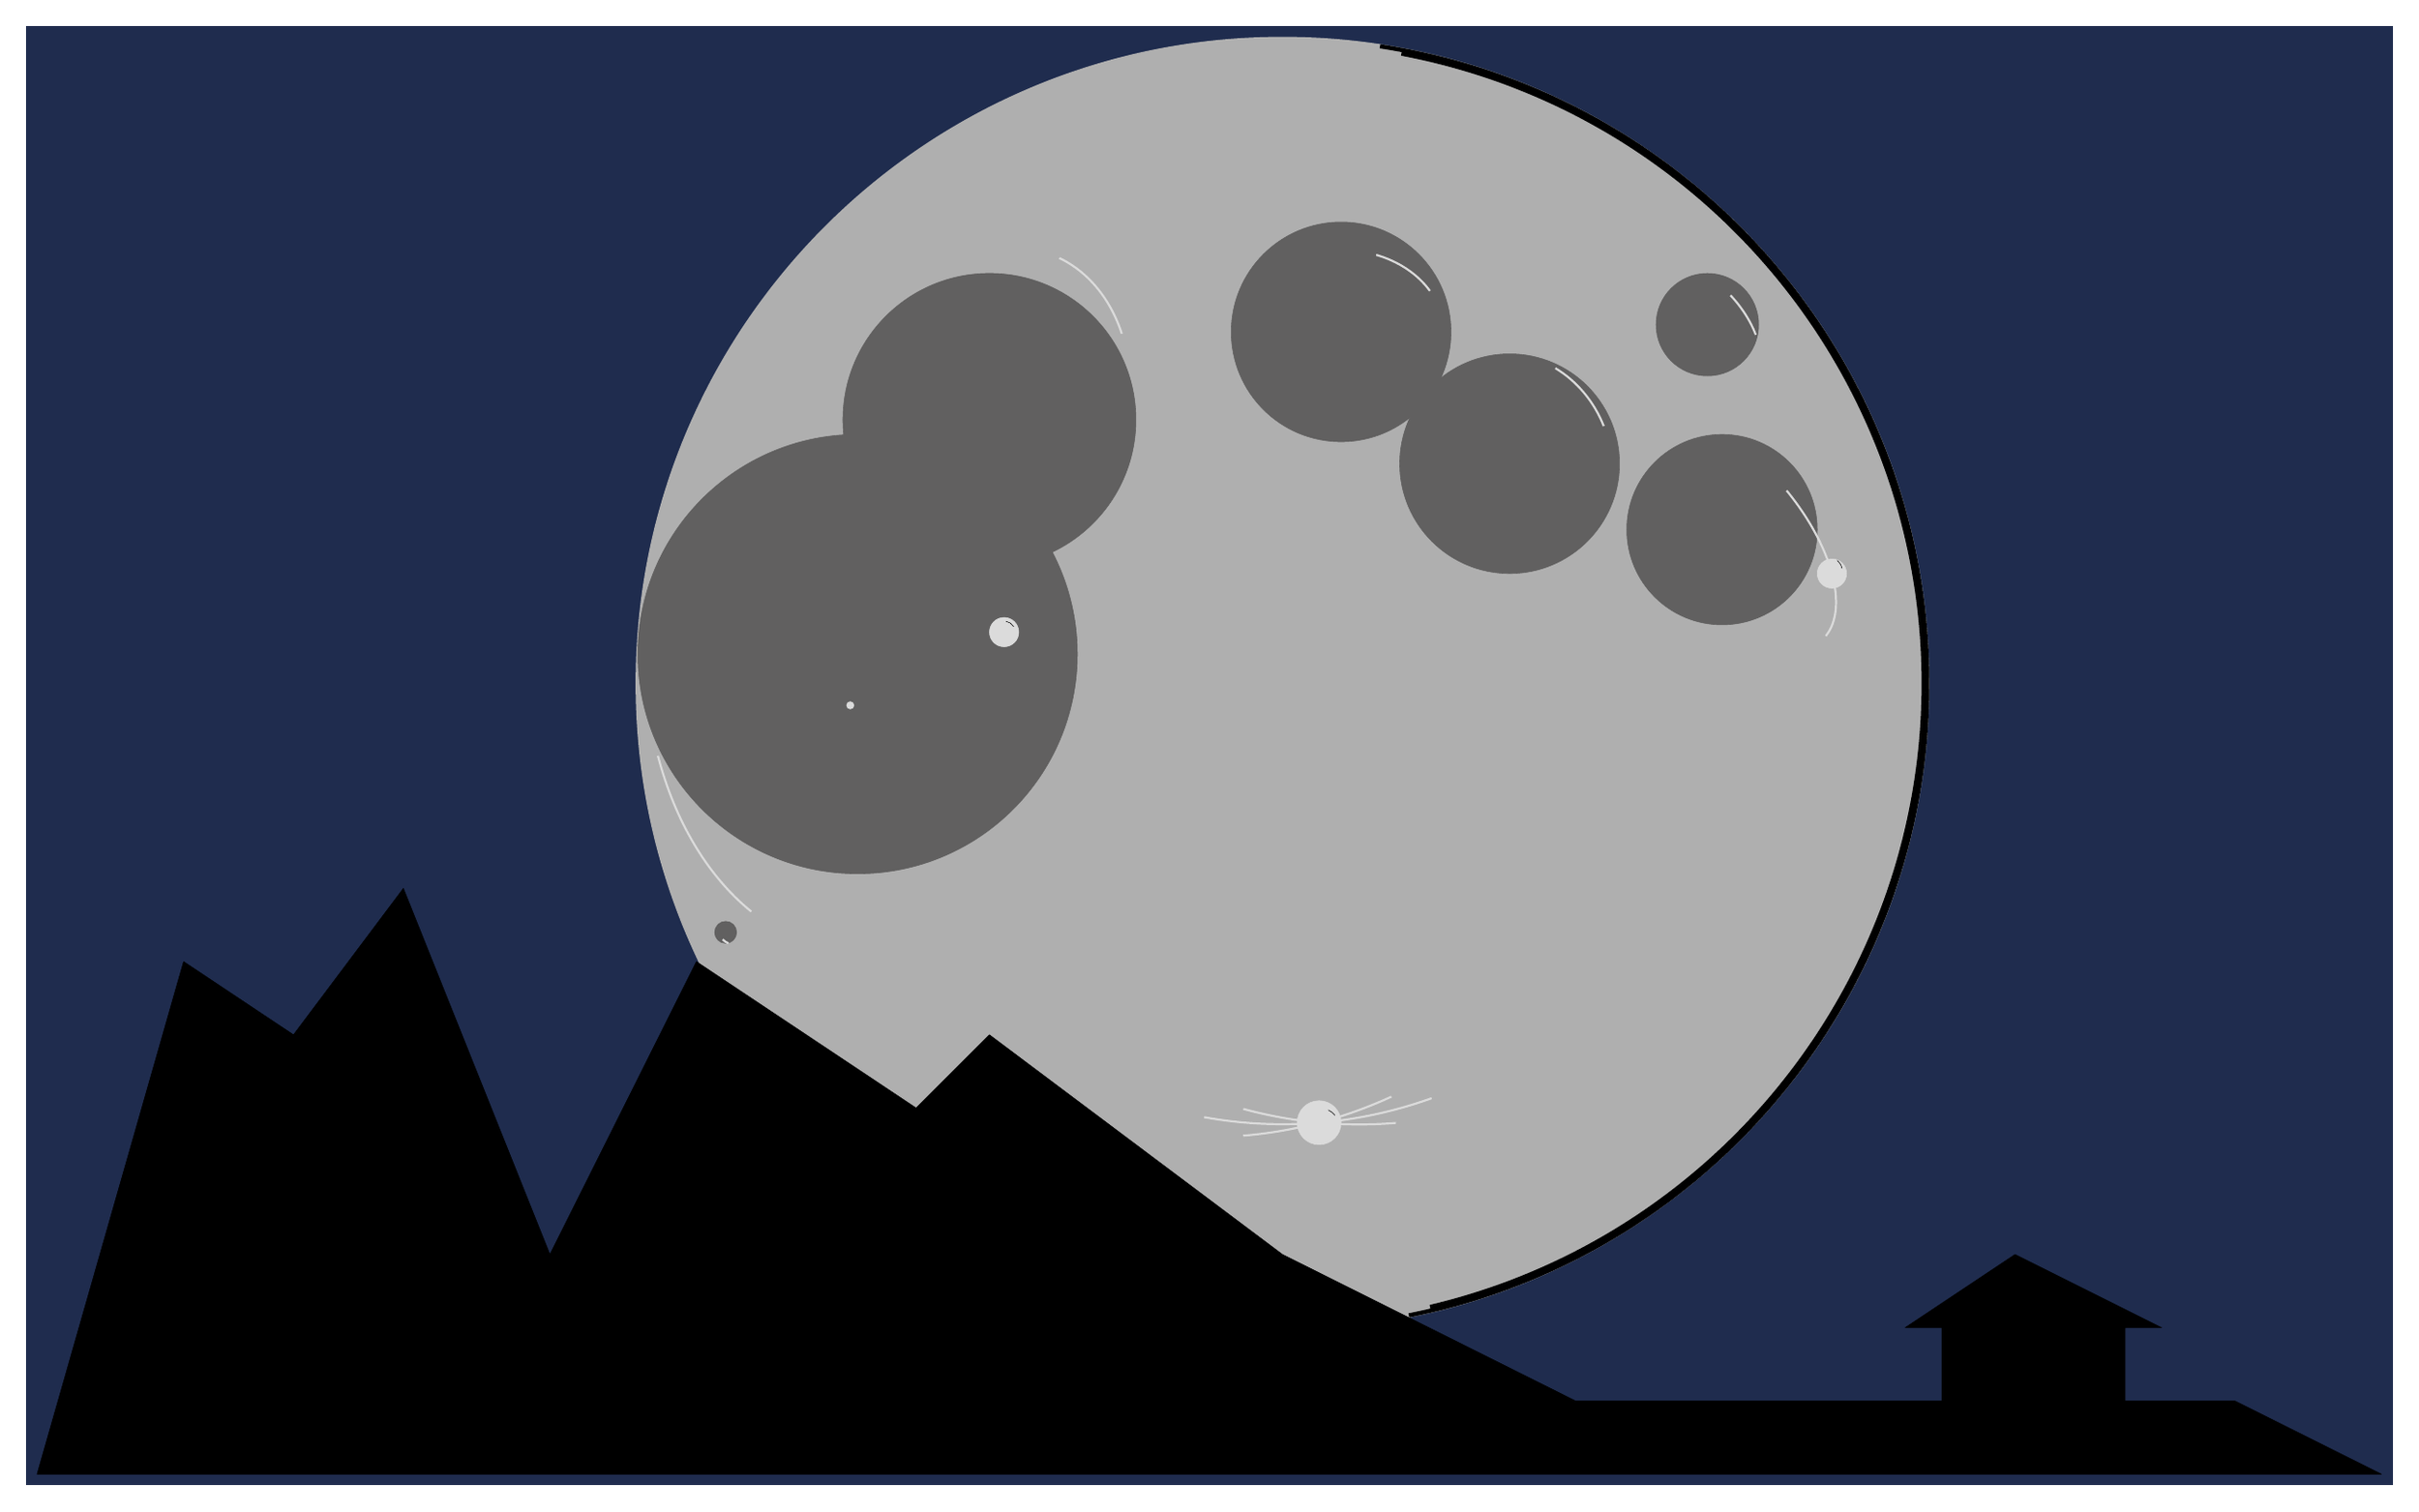
\begin{tikzpicture}[background rectangle/.style={fill=space},show background rectangle]
		%
		%moon
		\tkzDefPoint(15,-0.2){L}
		\tkzDefPoint(6.2,0){L1}
		\tkzDefShiftPoint[L1](0:17.6){La1}
		\tkzDefShiftPoint[L1](0:17.55){La2}
		\tkzDrawCircle[color=moon,fill=moon,ultra thick](L,L1)
		\tkzDrawArc[ultra thick, rotate](L,La1)(-80)
		\tkzDrawArc[ultra thick, rotate](L,La1)(80)
		\tkzDrawArc[ultra thick, rotate](L,La2)(-78)
		\tkzDrawArc[ultra thick, rotate](L,La2)(78)
		%
		\tkzDefPoint(15.5,-6.2){C3}
		\tkzDefShiftPoint[C3](0:0.3){Cr3}
		\tkzDefShiftPoint[Cr3](0:-0.05){Ca3}
		\tkzDrawArc[thick, color=linem, rotate](L,C3)(-15)
		\tkzDrawArc[thick, color=linem, rotate](L,C3)(15)
		\tkzDrawArc[rotate around={10:(C3)},thick, color=linem, rotate](L,C3)(-10)
		\tkzDrawArc[rotate around={10:(C3)},thick, color=linem, rotate](L,C3)(10)
		\tkzDrawArc[rotate around={-10:(C3)},thick, color=linem, rotate](L,C3)(-10)
		\tkzDrawArc[rotate around={-10:(C3)},thick, color=linem, rotate](L,C3)(10)
		\begin{scope}[yscale=0.8]
			\tkzDrawCircle[color=linem,fill=linem](C3,Cr3)
			\tkzDrawArc[rotate around={30:(C3)},rotate](C3,Ca3)(30)
		\end{scope}
		%
		\tkzDefPoint(7.4,-3.6){M1}
		\tkzDefShiftPoint[M1](0:0.15){Mr1}
		\tkzDefShiftPoint[Mr1](0:-0.05){Ma1}
		\begin{scope}[rotate around={30:(M1)},yscale=1.8]
			\tkzDrawCircle[color=craterm,fill=craterm](M1,Mr1)
			\tkzDrawArc[rotate around={220:(M1)},thick,color=linem,rotate](M1,Ma1)(40)
		\end{scope}
		%
		\tkzDefPoint(20.8,4.7){M2}
		\tkzDefShiftPoint[M2](0:0.7){Mr2}
		\tkzDefShiftPoint[Mr2](0:-0.1){Ma2}
		\begin{scope}[rotate around={40:(M2)},yscale=1.9]
			\tkzDrawCircle[color=craterm,fill=craterm](M2,Mr2)
			\tkzDrawArc[rotate around={-10:(M2)},thick,color=linem,rotate](M2,Ma2)(40)
		\end{scope}
		%
		\tkzDefPoint(15.8,4.6){M3}
		\tkzDefShiftPoint[M3](0:1.5){Mr3}
		\tkzDefShiftPoint[Mr3](0:-0.1){Ma3}
		\begin{scope}[yscale=0.8]
			\tkzDrawCircle[color=craterm,fill=craterm](M3,Mr3)
			\tkzDrawArc[rotate around={30:(M3)},thick,color=linem,rotate](M3,Ma3)(40)
		\end{scope}
		%
		\tkzDefPoint(18.1,2.8){M4}
		\tkzDefShiftPoint[M4](0:1.5){Mr4}
		\tkzDefShiftPoint[Mr4](0:-0.1){Ma4}
		\begin{scope}[rotate around={20:(M4)},yscale=1.1]
			\tkzDrawCircle[color=craterm,fill=craterm](M4,Mr4)
			\tkzDrawArc[rotate around={20:(M4)},thick,color=linem,rotate](M4,Ma4)(40)
		\end{scope}
		%
		\tkzDefPoint(22.5,1.3){C2}
		\tkzDefPoint(21,1.9){M5}
		\tkzDefShiftPoint[M5](0:1.3){Mr5}
		\begin{scope}[rotate around={42:(M5)},yscale=2]
			\tkzDrawCircle[color=craterm,fill=craterm](M5,Mr5)
			\tkzDrawArc[thick,color=linem,rotate](M5,C2)(40)
			\tkzDrawArc[thick,color=linem,rotate](M5,C2)(-40)
		\end{scope}
		%
		\tkzDefPoint(9.2,0.2){M6}
		\tkzDefShiftPoint[M6](0:3){Mr6}
		\tkzDefShiftPoint[Mr6](0:-0.1){Ma6}
		\begin{scope}[yscale=1.4]
			\tkzDrawCircle[color=craterm,fill=craterm](M6,Mr6)
			\tkzDrawArc[rotate around={-160:(M6)},thick,color=linem,rotate](M6,Ma6)(40)
		\end{scope}
		%
		\tkzDefPoint(11,3.4){M7}
		\tkzDefShiftPoint[M7](0:2){Mr7}
		\tkzDefShiftPoint[Mr7](0:-0.1){Ma7}
		\begin{scope}[rotate around={-20:(M7)},yscale=1.3]
			\tkzDrawCircle[color=craterm,fill=craterm](M7,Mr7)
			\tkzDrawArc[rotate around={30:(M7)},thick,color=linem,rotate](M7,Ma7)(40)
		\end{scope}
		%
		\tkzDefPoint(11.2,0.5){C1}
		\tkzDefShiftPoint[C1](0:0.2){Cr1}
		\tkzDefShiftPoint[Cr1](0:-0.05){Ca1}
		\tkzDrawCircle[color=linem,fill=linem](C1,Cr1)
		\tkzDrawArc[rotate around={30:(C1)},rotate](C1,Ca1)(50)
		%
		\tkzDefShiftPoint[C2](0:0.2){Cr2}
		\tkzDefShiftPoint[Cr2](0:-0.05){Ca2}
		\begin{scope}[yscale=1.4]
			\tkzDrawCircle[color=linem,fill=linem](C2,Cr2)
			\tkzDrawArc[rotate around={20:(C2)},rotate](C2,Ca2)(40)
		\end{scope}
		%
		\tkzDefPoint(9.1,-0.5){C4}
		\tkzDefShiftPoint[C4](0:0.05){Cr4}
		\begin{scope}[yscale=1.1]
			\tkzDrawCircle[color=linem,fill=linem](C4,Cr4)
		\end{scope}
		%
		% skyline
		\begin{scope}[shift={(0,-8)}]
			\tkzDefPoint(-2,-3){S1}
			\tkzDefPoint(0,4){S2}
			\tkzDefPoint(1.5,3){S3}
			\tkzDefPoint(3,5){S4}
			\tkzDefPoint(5,0){S5}
			\tkzDefPoint(7,4){S6}
			\tkzDefPoint(10,2){S7}
			\tkzDefPoint(11,3){S8}
			\tkzDefPoint(13,-2){S9}
			\tkzDefPoint(15,0){S10}
			\tkzDefPoint(19,-2){S11}
			%
			\tkzDefPoint(24,-2){S12}
			\tkzDefPoint(24,-1){S13}
			\tkzDefPoint(23.5,-1){S14}
			\tkzDefPoint(25,0){S15}
			\tkzDefPoint(27,-1){S16}
			\tkzDefPoint(26.5,-1){S17}
			\tkzDefPoint(26.5,-2){S18}
			\tkzDefPoint(28,-2){S19}
			\tkzDefPoint(30,-3){S20}
			\tkzDrawPolygon[fill=black](S1,S2,S3,S4,S5,S6,S7,S8,S10,S11,S12,S13,S14,S15,S16,S17,S18,S19,S20)
		\end{scope}
	\end{tikzpicture}
\end{document}